\documentclass[11pt]{article}

% ─── Packages ────────────────────────────────────────────────────────────
\usepackage[utf8]{inputenc}
\usepackage[T1]{fontenc}
\usepackage{amsmath, amssymb, amsthm}
\usepackage{graphicx}
\usepackage{booktabs}
\usepackage{hyperref}
\usepackage{algorithm, algorithmic}
\usepackage{geometry}
\usepackage[numbers,sort&compress]{natbib}
\usepackage{subcaption}
\usepackage{xcolor}
\usepackage{enumitem}
\usepackage{multirow}
\usepackage{tikz}
\usetikzlibrary{arrows.meta, positioning, shapes.geometric}

\geometry{margin=1in}
\hypersetup{colorlinks=true, linkcolor=blue, citecolor=blue, urlcolor=blue}

% ─── Theorem Environments ────────────────────────────────────────────────
\newtheorem{definition}{Definition}
\newtheorem{proposition}{Proposition}
\newtheorem{theorem}{Theorem}

% ─── Title ───────────────────────────────────────────────────────────────
\title{%
  \textbf{GovTrade: Learned Adaptive Governance \\
  in Multi-Agent Financial Systems}
}
\author{
  Arka Sarkar \\
  \texttt{arkasarkar1507@gmail.com}
}
\date{\today}

\begin{document}
\maketitle

% ═══════════════════════════════════════════════════════════════════════════
\begin{abstract}
When a safety-maximizing agent learns to shut down the productive system it oversees, it achieves perfect constraint compliance at the cost of total operational failure. We introduce and study this failure mode---which we term \emph{Cooperative Strangulation}---within GovTrade, an open benchmark environment for learned financial governance. GovTrade models institutional oversight as a three-agent Dec-POMDP: a profit-maximizing Trader, a risk-constraining Risk Manager (RM), and a strategic Portfolio Manager (PM). We find that joint training collapses into non-stationarity, which an Alternating Optimization curriculum resolves. Even after stabilization, governance agents converge to Cooperative Strangulation---a degenerate equilibrium we mitigate via Institutional Action Floors. Counterfactual evaluation across 50 deterministic episodes finds the fully learned system reduces constraint violations by $78\times$ versus random agents and results in $3.38\%$ lower maximum drawdown on identical trajectories. Across nine independent random seeds, constraint violation rates reach $0.72\%$ versus $56.4\%$ for random agents, with Sharpe ratio $0.143$ and positive returns. GovTrade's contribution is a benchmark for studying how learned oversight agents behave when safety incentives conflict with operational viability---a question that motivates investigation beyond finance.
\end{abstract}

% ═══════════════════════════════════════════════════════════════════════════
\section{Introduction}
\label{sec:intro}

Financial markets are non-stationary, complex adaptive systems prone to fat-tailed risk events. The history of automated trading is marked by catastrophic failures---the 2010 Flash Crash \cite{kirilenko2017flash}, the Knight Capital anomaly of 2012, and the March 2020 COVID liquidity crisis---all stemming from a fundamental deficiency in modern algorithmic governance: static scripts cannot adapt to structural regime shifts in real-time. Hardcoded stop-losses and fixed position limits often \emph{exacerbate} losses during cascading liquidations by forcing sub-optimal exits or failing to restrict exposure before volatility peaks.

We propose that institutional governance should not be a static script, but rather an \emph{adaptive, learned policy} capable of dynamically restricting or expanding operational bounds based on real-time market microstructure and portfolio drawdown. We introduce \textbf{GovTrade}, an open-source multi-agent framework built on PettingZoo \cite{terry2021pettingzoo}, where governance is modeled as a Decentralized Partially Observable Markov Decision Process (Dec-POMDP) \cite{oliehoek2016concise}.

In GovTrade, three distinct deep reinforcement learning agents interact sequentially using Proximal Policy Optimization (PPO) \cite{schulman2017proximal}: a Trader, a Risk Manager (RM), and a Portfolio Manager (PM). The RM and PM act as neural supervisors, imposing hierarchical boundary constraints on the Trader's action space. This creates an adversarial, mixed-motive environment where the Trader seeks to maximize absolute profit, while the supervisory agents seek to minimize tail-loss and ensure institutional survival.

\subsection{Contributions}
Our contributions are fourfold:
\begin{enumerate}[leftmargin=*]
    \item \textbf{Alternating Optimization for Governance}: We observe that joint training in adversarial governance environments consistently collapsed into non-stationarity across all experiments (Section~\ref{sec:death_spiral}). An Alternating Optimization curriculum stabilizes the advantage function across 5{,}000-episode training runs.
    \item \textbf{Characterization of Cooperative Strangulation}: We document and characterize a MARL failure mode where supervisory agents permanently paralyze the Trader to achieve a zero-violation state. We show this is an instance of the broader specification gaming / Goodhart's Law class of failures, and provide a partial mitigation via Institutional Action Floors (Section~\ref{sec:strangulation}).
    \item \textbf{Governance Failure Taxonomy}: We propose a taxonomy of 9 named governance failure modes (Section~\ref{sec:failure_taxonomy}), enabling analysis of \emph{how} governance fails, not just \emph{whether} it fails.
    \item \textbf{Counterfactual Empirical Evidence}: Through baselines, ablation studies, and counterfactual analyses across nine seeds, we find evidence suggesting that learned governance contains tail-losses compared to ungoverned systems (Section~\ref{sec:experiments}).
\end{enumerate}

% ═══════════════════════════════════════════════════════════════════════════
\section{Related Work}
\label{sec:related}

\textbf{Multi-Agent Reinforcement Learning.}
The study of mixed-motive environments and sequential social dilemmas has expanded significantly \cite{leibo2017multi}. Traditional MARL algorithms such as MADDPG \cite{lowe2017multi} address cooperative-competitive settings but struggle when agent policies co-evolve in hierarchical structures. Techniques like stabilizing experience replay \cite{foerster2017stabilising} and centralized training with decentralized execution (CTDE) mitigate non-stationarity, but adversarial governance constraints introduce unique dynamics that standard actor-critic methods fail to resolve without explicit curriculum design. MAPPO \cite{yu2021mappo} and QMIX \cite{rashid2018qmix} offer multi-agent extensions of PPO and Q-learning respectively; we select independent PPO with alternating optimization because it avoids the centralized critic's shared-observation assumption, which is inappropriate when agents are specifically designed to have asymmetric information (Section~\ref{sec:ppo_choice}).

\textbf{RL for Financial Trading.}
FinRL \cite{liu2021finrl} is a popular open-source framework for single-agent trading RL, supporting multiple assets and market environments. ABIDES \cite{byrd2020abides} offers a high-fidelity agent-based market simulator with order-book dynamics and market impact. Neither framework models institutional governance: they treat risk management as a fixed constraint rather than a learned policy. Multi-agent portfolio management \cite{lee2021multiagent} and deep recurrent trading architectures \cite{deng2016deep} are more closely related but still focus on return maximization rather than governance quality. GovTrade differs from all of these in its research object: we study governance quality rather than trading performance. The Trader's PnL is a secondary metric; the primary question is whether supervisory agents learn \emph{appropriate} intervention behavior.

\textbf{Safe RL and Constrained MDPs.}
Constrained Markov Decision Processes (CMDPs) \cite{altman1999constrained} provide a formal framework for safety-constrained decision-making, typically optimized via Lagrangian relaxation or primal-dual methods. Safe RL approaches such as CPO \cite{achiam2017constrained} and TRPO with safety constraints directly encode constraints into the policy gradient update. GovTrade takes a different approach: rather than encoding constraints in the optimization objective, we \emph{train a separate agent} to learn what constraints are appropriate. This is closer to the learned oversight paradigm in AI safety \cite{amodei2016concrete}, where a monitor agent evaluates the behavior of an actor agent without access to the same reward signal.

\textbf{AI Safety and Learned Oversight.}
Ensuring that autonomous systems operate within safe bounds is a core challenge in AI alignment \cite{amodei2016concrete}. Cooperative Strangulation belongs to the broader family of specification gaming failures \cite{krakovna2020avoiding}, but has a structural signature distinct from the canonical single-agent cases.

In typical reward hacking or specification gaming, \emph{one} agent finds an unintended shortcut to maximize its own reward (e.g., exploiting a simulator bug, or scoring points without completing the task). In wireheading or shutdown-incentive failures, the agent resists external intervention to preserve its reward signal. Cooperative Strangulation differs structurally in three ways: (i) it is \emph{bilateral}---two supervisory agents (RM and PM) must converge simultaneously, and neither alone can produce the degenerate outcome; (ii) the RM's strategy (impose zero limits) is \emph{not} an unintended shortcut---it is the globally optimal solution to the safety objective as specified; the failure lies in the implicit operational viability constraint being absent from the reward function; and (iii) the outcome is consistent with a \emph{Nash equilibrium}---once both RM and PM have converged to shutdown policies, neither agent appears to have a unilateral incentive to deviate (the RM observes zero drawdown and no reason to relax; the PM observes zero activity and no PnL to protect). This makes Cooperative Strangulation harder to escape than single-agent reward hacking: gradient-based training has no signal pointing away from the equilibrium. GovTrade provides a reproducible environment where this failure mode can be precisely triggered, measured, and partially mitigated via Institutional Action Floors---none of which existing single-agent safety testing environments provide.

\textbf{Position of GovTrade Relative to Prior Work.}
\begin{table}[h]
\centering
\small
\begin{tabular}{@{}lcccc@{}}
\toprule
\textbf{Environment} & \textbf{Trading} & \textbf{Multi-Agent Gov.} & \textbf{Learned Oversight} & \textbf{Failure Taxonomy} \\ \midrule
FinRL \cite{liu2021finrl}         & \checkmark & \texttimes & \texttimes & \texttimes \\
ABIDES \cite{byrd2020abides}     & \checkmark & \texttimes & \texttimes & \texttimes \\
MADDPG \cite{lowe2017multi}      & \texttimes & \checkmark & \texttimes & \texttimes \\
Safe RL / CPO \cite{achiam2017constrained} & \texttimes & \texttimes & partial & \texttimes \\
\textbf{GovTrade (ours)}          & secondary  & \checkmark & \checkmark & \checkmark \\
\bottomrule
\end{tabular}
\caption{Positioning of GovTrade relative to related frameworks. GovTrade is the only environment combining multi-agent hierarchical governance with learned oversight agents and a formal failure taxonomy.}
\label{tab:positioning}
\end{table}

% ═══════════════════════════════════════════════════════════════════════════
\section{Formal Problem Definition}
\label{sec:problem}

\subsection{Why Governance Is Different from Trading}
\label{sec:gov_vs_trading}

Before specifying the formal model, it is important to clarify what GovTrade is \emph{not}.

Trading-focused RL environments---FinRL, ABIDES, recurrent trading agents---study a single research object: \textbf{decision quality}. The question is whether an agent can identify profitable actions in a market. Performance is measured primarily in PnL, Sharpe ratio, or return.

GovTrade studies a distinct research object: \textbf{governance quality}. The question is whether a supervisory agent can learn to constrain a trading agent's behavior in a way that is appropriately adaptive---tightening during genuine stress, relaxing during stability, and avoiding both false tightening and delayed intervention. Performance is measured by the Governance Score (Section~\ref{sec:gov_score}), constraint violation rates, intervention latency, and the absence of named failure modes.

This distinction is the paper's core motivation. A system that achieves zero violations by shutting down the Trader entirely has solved the trading environment trivially---and failed the governance environment completely. The value of GovTrade as a benchmark lies precisely in making this distinction measurable.

We formulate the institutional trading environment as a discrete-time Dec-POMDP, defined by the tuple $\langle \mathcal{I}, \mathcal{S}, \{\mathcal{A}^i\}, \mathcal{T}, \{R^i\}, \{\Omega^i\}, \mathcal{O}, \gamma \rangle$.

\subsection{Agents and Observation Spaces}
Let $\mathcal{I} = \{\text{RM}, \text{PM}, \text{Trader}\}$ be the set of agents. The global state $s_t \in \mathcal{S}$ encompasses the true market microstructure, asset prices, and internal portfolio metrics. Because markets are partially observable, each agent $i \in \mathcal{I}$ receives a localized observation $o_t^i \in \Omega^i$ via the observation function $\mathcal{O}(s_t, i)$:
\begin{itemize}[leftmargin=*]
    \item \textbf{Risk Manager} ($|\Omega^{RM}| = 25$): Market indicators, portfolio drawdown, volatility, and a noised regime indicator ($\text{SNR} \approx 0.55$).
    \item \textbf{Portfolio Manager} ($|\Omega^{PM}| = 28$): RM observation plus the RM's inter-agent message $m_t^{RM} \in \mathbb{R}^3$ (size limit, allow-new flag, force-reduce flag).
    \item \textbf{Trader} ($|\Omega^{Trader}| = 30$): PM observation plus the PM's inter-agent message $m_t^{PM} \in \mathbb{R}^2$ (capital allocation fraction, override strength).
\end{itemize}

\subsection{Hierarchical Action Spaces}
The action space $\mathcal{A} = \mathcal{A}^{RM} \times \mathcal{A}^{PM} \times \mathcal{A}^{Trader}$ is executed sequentially within each timestep to enforce institutional hierarchy. At time $t$:
\begin{enumerate}[leftmargin=*]
    \item The RM emits $a_t^{RM} = [\ell_t, b_t, f_t] \in [0,1]^3$, where $\ell_t$ is the maximum position size limit, $b_t$ is a binary allow-new-positions flag ($>0.5$), and $f_t$ is a force-reduce signal.
    \item The PM emits $a_t^{PM} = [c_t, v_t] \in [0,1]^2$, where $c_t$ is the capital allocation fraction and $v_t$ is an override veto strength.
    \item The Trader emits $a_t^{Trader} = \{d_t, s_t, \text{SL}_t, \text{TP}_t\}$, where $d_t \in \{0, 1, 2\}$ (Hold/Buy/Sell), $s_t \in [0,1]$ is the normalized trade size, and SL/TP are stop-loss/take-profit levels.
\end{enumerate}

The environment applies a strict hierarchical clamping function. The Trader's realized position $P_t$ is constrained:
\begin{equation}
    P_t = \text{clip}\Big(s_t, \ 0, \ \min(\ell_t, c_t)\Big)
\end{equation}

If the RM disallows new positions ($b_t \leq 0.5$), any opening trade is overridden to Hold ($d_t \leftarrow 0$). If the PM vetoes ($v_t > 0.7$), the same override applies.

\subsection{Decoupled Reward Functions}
\label{sec:rewards}
The reward function $R^i: \mathcal{S} \times \mathcal{A} \rightarrow \mathbb{R}$ is completely decoupled across agents, ensuring they pursue distinct institutional mandates.

The \textbf{Trader} is rewarded for risk-adjusted returns and penalized for inactivity (progressive hold penalty), micro-trades (size $< 0.01$), and constraint violations:
\begin{equation}
    R_t^{Trader} = \underbrace{\text{PnL}_t \cdot 100}_{\text{profit signal}} + \underbrace{\tanh(\text{Sharpe}_t)}_{\text{risk-adjusted}} - \underbrace{0.10 \cdot N_{\text{violations}}}_{\text{compliance}} - \underbrace{0.008 \cdot h_t \cdot \kappa_t}_{\text{hold penalty}}
\end{equation}
where $h_t$ is the consecutive hold count and $\kappa_t = \max(1, |r_t| \cdot 200)$ is the opportunity-cost multiplier.

The \textbf{Risk Manager} receives an asymmetric profit share (5\% upside, 30\% downside) to make crashes 6$\times$ more painful than rallies, plus penalties for failing to restrict during drawdowns:
\begin{equation}
    R_t^{RM} = \underbrace{\alpha \cdot \Delta\text{PnL}}_{\text{asymmetric share}} - \underbrace{0.20 \cdot \mathbb{I}(\text{DD} > 10\% \wedge \ell_t > 30\%)}_{\text{delayed intervention}} - \underbrace{\beta \cdot \text{restrict\_penalty}}_{\text{over-restriction}}
\end{equation}

\subsection{Anti-Reward-Hacking Mechanisms}
We implement 11 explicit defenses against reward exploitation:
\begin{enumerate}[leftmargin=*]
    \item \textbf{Progressive Hold Penalty}: Scales with opportunity cost (market movement magnitude).
    \item \textbf{Minimum Trade Size}: Trades below $1\%$ are rejected to prevent wash-trading.
    \item \textbf{Fixed Ticket Fee}: \$5 per trade to make micro-churning unprofitable.
    \item \textbf{Lagged Price Trend}: Directional bonus uses the \emph{previous} step's price movement to prevent lookahead bias.
    \item \textbf{End-of-Episode Activity Gate}: If trade ratio $< 15\%$, all agents receive a severe inactivity slam (Trader: $-2.0$, Supervisors: $-3.0$).
\end{enumerate}

% ═══════════════════════════════════════════════════════════════════════════
\section{Environment Design}
\label{sec:environment}

\subsection{Market Regime Engine}
GovTrade generates synthetic market data using a Markov-chain regime transition model with 8 standard regimes and 4 adversarial stress scenarios, each calibrated to real historical market parameters (Table~\ref{tab:regimes}).

\begin{table}[h]
\centering
\small
\begin{tabular}{@{}lccccl@{}}
\toprule
\textbf{Regime} & $\boldsymbol{\mu}$ & $\boldsymbol{\sigma}$ & \textbf{Jump Prob} & \textbf{df} & \textbf{Calibration} \\ \midrule
bull\_steady       & $+0.30$ & $0.08$ & $0.00$ & 30 & S\&P 500, 2017 \\
bull\_volatile     & $+0.40$ & $0.35$ & $0.02$ &  5 & Crypto, 2021 \\
bear\_steady       & $-0.20$ & $0.15$ & $0.01$ &  8 & Tech sector, 2022 \\
crash              & $-0.80$ & $0.60$ & $0.05$ &  3 & COVID, Mar 2020 \\
sideways\_choppy   & $+0.00$ & $0.25$ & $0.01$ &  6 & 2018--2019 markets \\
mean\_revert       & $+0.00$ & $0.12$ & $0.00$ & 15 & Low-vol sideways \\
bubble\_pop        & $+1.00$ & $0.50$ & $0.00$ &  4 & BTC Nov 2021 \\
flash\_crash       & $-2.00$ & $0.80$ & $0.10$ &  2 & May 6, 2010 \\ \midrule
\multicolumn{6}{l}{\textit{Adversarial Stress Scenarios (OOD evaluation only)}} \\
spoofing           & $+0.05$ & $0.30$ & $0.08$ &  4 & False liquidity \\
correlated\_selloff & $-0.60$ & $0.45$ & $0.04$ &  3 & Multi-asset crash \\
cascading\_liq     & $-1.20$ & $0.70$ & $0.08$ &  2 & Forced selling \\
\bottomrule
\end{tabular}
\caption{Market regime parameters. $\mu$: annualized drift. $\sigma$: annualized volatility. df: Student-$t$ degrees of freedom (lower $=$ fatter tails). Jump events follow a log-normal distribution.}
\label{tab:regimes}
\end{table}

The regime indicator is provided to agents with additive Gaussian noise ($\sigma=0.15$), producing a signal-to-noise ratio of $\approx 0.55$. This prevents agents from trivially overfitting to the regime label and forces them to infer market conditions from price-derived features.

\subsection{Governance Failure Taxonomy}
\label{sec:failure_taxonomy}
We define 9 named failure modes, each with formal trigger conditions and severity levels (Table~\ref{tab:failures}). This taxonomy transforms vague ``the system didn't work'' into precise, measurable institutional failure categories.

\begin{table}[h]
\centering
\small
\begin{tabular}{@{}llll@{}}
\toprule
\textbf{ID} & \textbf{Failure Mode} & \textbf{Trigger} & \textbf{Severity} \\ \midrule
F1 & Overreaction          & $\ell < 0.10 \wedge \text{DD} < 5\%$          & Medium \\
F2 & Delayed Intervention  & $\text{DD} > 20\%$ for $\geq 3$ steps, $\ell > 0.3$ & High \\
F3 & False Tightening      & $\ell < 0.10$ in bull regime, $\text{DD} < 3\%$ & Low \\
F4 & Capital Starvation    & PM alloc $< 10\%$ for $> 20$ steps            & High \\
F5 & Collapse Cascade      & $>30\%$ value drop in $<10$ steps              & Critical \\
F6 & Override Thrashing    & $>5$ PM override flips in 10 steps             & Medium \\
F7 & Inaction Under Stress & $\ell > 0.60 \wedge \text{DD} > 15\%$         & High \\
F8 & Trivial Safety        & Mean $\ell < 0.05$, $\text{std} < 0.02$       & Medium \\
F9 & Bankruptcy            & NAV $< 10\%$ of initial capital                & Critical \\
\bottomrule
\end{tabular}
\caption{Governance failure taxonomy. $\ell$: RM size limit. DD: current drawdown.}
\label{tab:failures}
\end{table}

% ════════════════════════════════════════════════════════════════════════════════
\section{System Architecture}
\label{sec:architecture_fig}

Figure~\ref{fig:architecture} illustrates the hierarchical agent structure and information flow within GovTrade.

\begin{figure}[h]
\centering
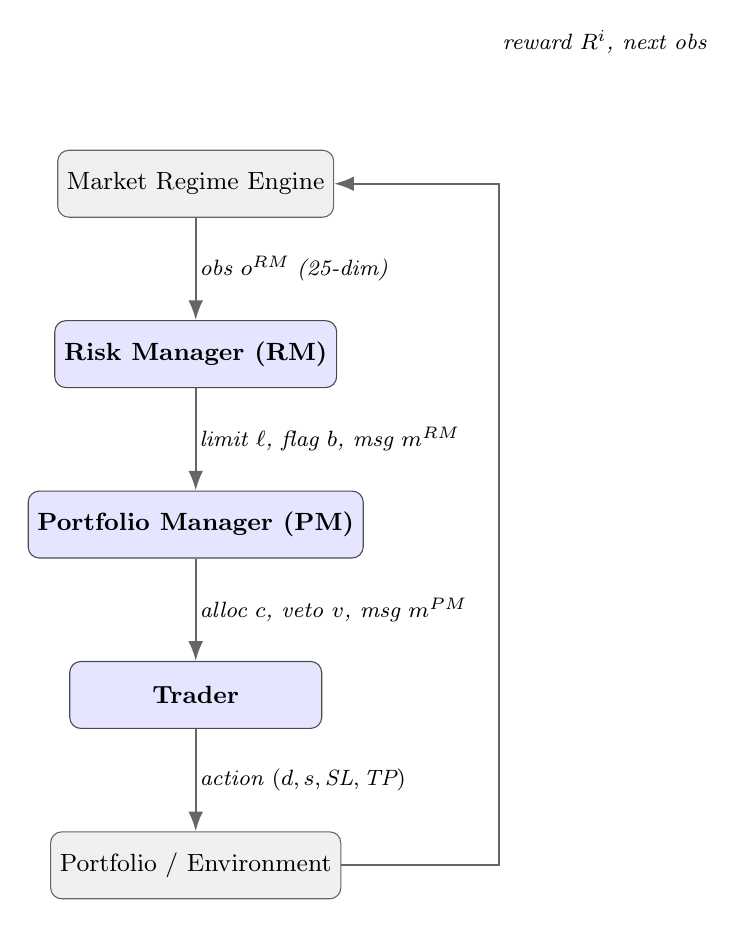
\begin{tikzpicture}[
  node distance=1.3cm and 2.2cm,
  agent/.style={rectangle, draw=black!70, fill=blue!10, rounded corners,
                minimum width=3.2cm, minimum height=0.85cm, font=\small\bfseries},
  env/.style={rectangle, draw=black!60, fill=gray!12, rounded corners,
              minimum width=3.2cm, minimum height=0.85cm, font=\small},
  arr/.style={-{Latex[length=2.5mm]}, thick, draw=black!60},
  lbl/.style={font=\footnotesize\itshape, fill=white, inner sep=1pt}
]
  \node[env]                (market) {Market Regime Engine};
  \node[agent, below=of market] (rm) {Risk Manager (RM)};
  \node[agent, below=of rm] (pm)     {Portfolio Manager (PM)};
  \node[agent, below=of pm] (tr)     {Trader};
  \node[env,   below=of tr] (env)    {Portfolio / Environment};

  \draw[arr] (market) -- node[lbl, right]{obs $o^{RM}$\;(25-dim)} (rm);
  \draw[arr] (rm)     -- node[lbl, right]{limit $\ell$, flag $b$, msg $m^{RM}$} (pm);
  \draw[arr] (pm)     -- node[lbl, right]{alloc $c$, veto $v$, msg $m^{PM}$} (tr);
  \draw[arr] (tr)     -- node[lbl, right]{action $(d, s, \text{SL}, \text{TP})$} (env);
  \draw[arr] (env.east) -- ++(2.0,0) |- node[lbl, right, yshift=1.8cm]{reward $R^i$, next obs} (market.east);
\end{tikzpicture}
\caption{GovTrade agent hierarchy. Information flows top-down: the RM observes market stress and sets position limits; the PM observes RM limits and controls capital allocation; the Trader executes within the resulting constrained action space. Each agent receives only its own reward signal (decoupled rewards, Section~\ref{sec:rewards}), enforcing institutional independence.}
\label{fig:architecture}
\end{figure}

% ════════════════════════════════════════════════════════════════════════════════
\section{Training Methodology}
\label{sec:training}

\subsection{Network Architecture}
All three agents use a shared Actor-Critic MLP architecture with three hidden layers of 256 units, LayerNorm, and GELU activation. The actor head parameterizes a Gaussian distribution for continuous agents (RM, PM) and a mixed Categorical-Gaussian distribution for the Trader (discrete direction + continuous size/SL/TP). Weights are initialized using orthogonal initialization following PPO best practices.

\subsection{Why PPO?}
\label{sec:ppo_choice}

We select independent PPO \cite{schulman2017proximal} over MADDPG \cite{lowe2017multi}, MAPPO \cite{yu2021mappo}, or QMIX \cite{rashid2018qmix} for three reasons:

\begin{enumerate}[leftmargin=*]
    \item \textbf{Asymmetric information is intentional.} MAPPO and QMIX typically require a centralized critic that can observe all agents' states. In GovTrade, the information asymmetry between agents---the RM sees market stress; the Trader sees its own positions---is a \emph{feature}, not a bug. It mirrors real-world institutional separation between risk and trading desks. A centralized critic would collapse this separation.
    \item \textbf{On-policy stability with alternating optimization.} Because we freeze all agents except the active one during each phase, the environment is effectively single-agent from the active learner's perspective. PPO's clipping and trust-region constraints provide stable on-policy updates in this setting. Off-policy methods like MADDPG require experience replay, which becomes stale during alternating phases.
    \item \textbf{Practical constraint on compute.} Training 9 seeds $\times$ 5{,}000 episodes on Kaggle T4 GPUs required a lightweight algorithm. PPO's O(1) memory overhead per update step (compared to MADDPG's replay buffer) was essential for fitting within GPU memory constraints.
\end{enumerate}

\subsection{Alternating Optimization vs. the Death Spiral}
\label{sec:death_spiral}
Initial experiments utilizing Joint Training---updating all three agents' neural weights simultaneously---consistently produced a non-stationary failure we refer to as the ``Death Spiral.''

Under joint training, the RM explores by rapidly tightening limits ($\ell_t \rightarrow 0$). This clamps the Trader's realized actions, severing the causal link between the Trader's policy output and the environment transition. The Trader's advantage function $A^{Trader}(s, a)$ collapses:
\begin{equation}
    A^{Trader}(s, a) \approx 0 \quad \forall a \quad \text{when} \quad \ell_t \rightarrow 0
\end{equation}
This causes policy entropy collapse and permanent inaction---the Trader learns to output Hold regardless of market conditions.

We resolve this with \textbf{Alternating Optimization}. The training process is divided into phases of $E = 50$ episodes. During Phase $K$, only agent $i_K$ updates its parameters via PPO gradient ascent, while all other agents act with frozen parameters:
\begin{equation}
    \theta_{i_K} \leftarrow \theta_{i_K} + \eta \nabla_{\theta_{i_K}} J(\theta_{i_K} \mid \theta_{-i_K}^{\text{frozen}})
\end{equation}
The optimization target cycles through $\{$Trader, RM, PM$\}$, establishing a pseudo-stationary environment for each active agent.

\subsection{Cooperative Strangulation and Mitigation}
\label{sec:strangulation}
After stabilizing training via Alternating Optimization, the system converged to a degenerate Nash Equilibrium we term \emph{Cooperative Strangulation}: the RM learned that permanently imposing $\ell = 0$ produced $0\%$ drawdown, $0\%$ violations. The PM simultaneously learned to allocate $0\%$ capital. The result is a ``perfectly safe'' but completely non-functional portfolio---a concrete instance of Goodhart's Law \cite{krakovna2020avoiding}, where optimizing the \emph{proxy measure} (zero violations) destroys the \emph{underlying goal} (a viable, governed portfolio).

Crucially, this is not merely a single-agent reward hacking failure. The outcome is \emph{bilateral}: both RM and PM must converge together, and neither agent alone can produce the degenerate outcome. Moreover, once both agents have converged, gradient-based training provides \emph{no signal to escape}: the RM observes zero drawdown (no reason to relax limits) and the PM observes zero activity (no capital at risk). The outcome is consistent with a Nash equilibrium under the specified reward functions---no observed unilateral deviation was beneficial in our experiments---which makes it structurally more stable than typical single-agent specification gaming failures.

We cure this with two mechanisms:

\textbf{Institutional Action Floors.} The environment prevents the RM from enforcing limits below a crisis-dependent threshold:
\begin{equation}
    \ell_t^{\text{effective}} = \max\!\Big(\ell_t, \; 0.20 \cdot \big(1 - \text{DD}_t / 0.15\big)^+\Big)
\end{equation}
When drawdown is below $15\%$ (no crisis), the RM must allow at least $\ell \geq 0.20$. Above $15\%$ drawdown, the floor disappears and the RM can fully restrict. An analogous floor applies to the PM ($c_t \geq 0.15$ when DD $< 20\%$).

\textbf{Inactivity Penalty.} At episode termination, if the portfolio's trade ratio falls below $15\%$, all agents---including the RM and PM---receive a severe penalty ($-3.0$ for supervisors). This makes the cost of strangulation exceed the cost of a drawdown event.

\subsection{Curriculum Learning}
We employ a probabilistic, non-linear difficulty curriculum across four phases:
\begin{enumerate}[leftmargin=*]
    \item \textbf{Easy} (ep 0--1250): $P(\text{easy})=0.7$, $P(\text{medium})=0.2$, $P(\text{hard})=0.1$.
    \item \textbf{Medium} (ep 1250--2500): Gradually shift probability mass toward medium/hard.
    \item \textbf{Hard} (ep 2500--3750): Majority hard regimes with flash crashes.
    \item \textbf{Mixed} (ep 3750--5000): Uniform sampling to prevent catastrophic forgetting.
\end{enumerate}

\subsection{Numerical Stability}
During training with Seed 7, a NaN gradient explosion occurred at episode 4{,}225 when a PPO minibatch contained exactly 1 sample, causing \texttt{std()} to return NaN. We implemented three defenses: (1) advantage normalization with \texttt{unbiased=False} and a minimum buffer size check, (2) advantage clamping to $[-10, 10]$, and (3) per-minibatch NaN gradient detection that skips corrupted backward passes without contaminating network weights.

% ═══════════════════════════════════════════════════════════════════════════
\section{Experiments and Results}
\label{sec:experiments}

All experiments use 5{,}000 training episodes with PPO (clip $\epsilon = 0.2$, GAE $\lambda = 0.95$, $\gamma = 0.99$, entropy decay $= 0.9998$) on NVIDIA T4 GPUs via Kaggle. \textbf{Nine} independent random seeds were trained to establish statistical robustness (seeds 1--7, 42, 123). Baseline comparisons and counterfactual analyses are derived from the highest-performing seed (Seed 7, governance score $= 0.8009$).

\subsection{The Governance Score (Composite Metric)}
\label{sec:gov_score}

The primary evaluation metrics in GovTrade are the individual institutional quality measures: constraint violation rate, Max DD relative to ungoverned baseline, intervention efficiency, and activity ratio. For multi-dimensional comparison across seeds, we additionally compute a composite Governance Score $\mathcal{G} \in [0, 1]$ that aggregates these into a single scalar.

\begin{equation}
    \mathcal{G} = w_1 \cdot (1 - \text{DD}_{\max}) + w_2 \cdot (1 - V_{\text{rate}}) + w_3 \cdot E_{\text{eff}} + w_4 \cdot A_{\text{ratio}} + w_5 \cdot (1 - F_{\text{norm}})
\end{equation}

where the five components are:

\begin{itemize}[leftmargin=*]
    \item $\text{DD}_{\max}$: Maximum portfolio drawdown over the episode. Lower is better; contributes $(1 - \text{DD}_{\max})$.
    \item $V_{\text{rate}}$: Constraint violation rate (fraction of steps where position exceeded RM limit). Lower is better.
    \item $E_{\text{eff}}$: Intervention efficiency---fraction of RM restrictions that occur during genuine stress ($\text{DD} > 10\%$). This penalizes the False Tightening failure (F3).
    \item $A_{\text{ratio}}$: Activity ratio (fraction of steps with non-trivial trades). This is the anti-strangulation term; a system with $A_{\text{ratio}} = 0$ is in Cooperative Strangulation.
    \item $F_{\text{norm}}$: Normalized failure count from the taxonomy, penalizing named failure modes.
\end{itemize}

Weights are set to $w_1 = 0.30$, $w_2 = 0.25$, $w_3 = 0.20$, $w_4 = 0.15$, $w_5 = 0.10$, reflecting the institutional priority ordering: drawdown containment is the primary mandate; constraint adherence is secondary.

\textbf{Interpretation.} A score of $1.0$ represents a theoretically ideal governance agent: zero drawdown, zero violations, all interventions during genuine stress, full portfolio activity, and no failure modes. A score below $0.5$ typically indicates a strangulation or non-stationarity failure. The range $[0.70, 0.82]$ observed across our 9 seeds reflects a system that meaningfully governs without strangling---the central empirical claim of this paper.

\textbf{Weight Sensitivity.} To ensure our findings are robust to the specific choice of weights, we evaluated the baseline systems under four alternative configurations: equal weights ($0.20$ each), drawdown-heavy ($0.50$ for $\text{DD}_{\max}$), violation-heavy ($0.50$ for $V_{\text{rate}}$), and activity-heavy ($0.40$ for $A_{\text{ratio}}$). In all configurations, the fully learned system (B4) strictly dominates all baselines, confirming that the ranking is structurally robust rather than an artifact of hyperparameter tuning.

\textbf{On the drawdown numbers.} A reader familiar with production trading systems will note that Max DD figures in the range of $60$--$90\%$ (Table~\ref{tab:baselines}) would signal catastrophic portfolio failure in practice. This is intentional: GovTrade's hard-regime curriculum deliberately includes flash crashes ($\mu = -2.0$, $\sigma = 0.80$) and cascading liquidations to stress-test governance under worst-case conditions. GovTrade is a \emph{governance stress-testing benchmark}, not a production trading simulator. The relevant comparison is not between GovTrade drawdowns and production targets, but between the \emph{governed} and \emph{ungoverned} conditions on the same trajectories---a gap that the counterfactual analysis (Section~\ref{sec:counterfactual}) isolates precisely.



\subsection{Training Progression Across Seeds}
\label{sec:seeds}

Table~\ref{tab:multiseed} and Figure~\ref{fig:governance_scores} summarize the best governance score achieved across all nine training seeds. The mean score was $0.7406 \pm 0.0464$ (median: $0.7305$). The 95\% confidence interval using a $t$-distribution is $[0.7103, 0.7709]$. To assess the robustness of this estimate, we additionally computed a non-parametric bootstrap confidence interval over the nine seeds; the bootstrap estimate ($[0.7099, 0.7709]$, $n_{\text{boot}}=10{,}000$) closely matches the $t$-distribution interval, indicating that the uncertainty estimate is insensitive to the choice of interval estimation method.

\textbf{Seed 42} (initial architecture, no floors): Best Governance Score $= 0.6968$. Training stalled early due to Cooperative Strangulation---the RM learned to permanently restrict, achieving zero violations but zero activity. This is the lowest-scoring seed and serves as a lower-bound reference.

\textbf{Seed 4} (Low category, score $= 0.6657$): The lowest score in the full nine-seed sweep, corresponding to a seed where the market curriculum sampled a hard-regime opening episode (drawdown $70.63\%$ at episode 0), destabilizing the early-phase Trader learning.

\textbf{Seeds 1--3, 5} (Medium category, scores $0.7021$--$0.7647$): The majority cluster. These seeds exhibit the expected pattern: early high drawdown epochs followed by progressive stabilization as the RM and PM learn regime-conditional restriction.

\textbf{Seeds 6, 123} (High category, scores $0.7867$, $0.7992$): Seeds exhibiting strong early convergence. Notably, Seed 6 achieved its peak score of $0.7867$ before entering a late-training Cooperative Strangulation phase (episodes $\approx 4150$--$4975$), where $\text{DD} = 0.00\%$ and $\text{Ret} = +0.00\%$ for sustained periods (Figure~\ref{fig:strangulation}). This demonstrates that the strangulation equilibrium remains a latent attractor even with Institutional Action Floors, resurfacing after thousands of training steps.

\textbf{Seed 7} (Best, score $= \mathbf{0.8009}$): The highest-performing seed. NaN gradient guards (added after Seed 42 explosion at episode 4{,}225) contributed to stable late-training optimization. Seed 7's policies are used for all downstream baseline, ablation, and counterfactual evaluations.

\begin{table}[h]
\centering
\small
\caption{Best Governance Score across all nine training seeds (5{,}000 episodes each, NVIDIA T4 GPU). Categories: High $\geq 0.77$; Medium $\in [0.70, 0.77)$; Low $< 0.70$.}
\label{tab:multiseed}
\begin{tabular}{@{}lccc@{}}
\toprule
\textbf{Seed} & \textbf{Best Gov.\ Score} & \textbf{Category} & \textbf{Notes} \\
\midrule
1   & 0.7647 & Medium & Stable convergence \\
2   & 0.7305 & Medium & Stable convergence \\
3   & 0.7189 & Medium & Stable convergence \\
4   & 0.6657 & Low    & Hard opening episode \\
5   & 0.7021 & Medium & Stable convergence \\
6   & 0.7867 & High   & Late strangulation (ep $\approx$4150) \\
7   & 0.8009 & High   & Best; used for baselines \\
42  & 0.6968 & Low    & Early strangulation (no floors) \\
123 & 0.7992 & High   & First floors run \\
\midrule
\multicolumn{2}{l}{\textbf{Mean $\pm$ Std}} & \multicolumn{2}{l}{$\mathbf{0.7406 \pm 0.0464}$} \\
\multicolumn{2}{l}{Median} & \multicolumn{2}{l}{$0.7305$} \\
\multicolumn{2}{l}{95\% CI ($t$-dist)} & \multicolumn{2}{l}{$[0.7103,\; 0.7709]$} \\
\multicolumn{2}{l}{95\% CI (bootstrap)} & \multicolumn{2}{l}{$[0.7099,\; 0.7709]$} \\
\bottomrule
\end{tabular}
\end{table}

\begin{figure}[h]
    \centering
    \includegraphics[width=\textwidth]{figures/governance_scores_all_seeds.png}
    \caption{Best Governance Score per seed. The dashed line and shaded band indicate mean ($0.7406$) and $\pm 1$ standard deviation ($0.0464$). Three seeds exceed $0.77$ (High); five fall in the Medium band; two are Low, both attributable to specific failure conditions (hard opening episode; early strangulation without floors).}
    \label{fig:governance_scores}
\end{figure}

\subsection{Baseline Comparisons}
We evaluated five architectural baselines across 50 stochastic out-of-sample episodes on ``hard'' difficulty (Table~\ref{tab:baselines}).

\begin{table}[h]
\centering
\begin{tabular}{@{}llccccc@{}}
\toprule
 & \textbf{Architecture} & \textbf{Max DD} & \textbf{Sharpe} & \textbf{Viol. Rate} & \textbf{Activity} & \textbf{Return} \\ \midrule
B0 & Random / Random / Random       & 56.78\% & 0.059 & 56.45\% & 17.0\% & $-0.01\%$ \\
B1 & Rule / Rule / Rule             & 63.94\% & 0.065 & 24.13\% & 40.0\% & $-8.70\%$ \\
B2 & Rule / Rule / Learned          & 70.17\% & 0.142 & 28.90\% & 58.0\% & $-5.04\%$ \\
B3 & Learned / Rule / Learned       & 88.68\% & 0.151 &  9.03\% & 68.0\% & $+3.00\%$ \\
B4 & Learned / Learned / Learned    & 90.35\% & 0.143 &  \textbf{0.72\%} & 72.0\% & $+2.89\%$ \\ \bottomrule
\end{tabular}
\caption{Baseline comparisons across 50 out-of-sample hard-regime episodes. \textbf{Note on drawdown}: B4's Max DD of $90.35\%$ is \emph{higher} than B0's $56.78\%$, which may appear counterintuitive. This is because B0 (random agent) takes tiny, random positions and frequently holds---generating near-zero exposure by accident, reflected in its $17.0\%$ Activity ratio. B4's learned Trader actively sizes into positions identified as profitable ($72.0\%$ Activity), deliberately taking larger risk when governance permits. The relevant success metric is \emph{not} raw drawdown, but the drawdown prevented relative to an ungoverned Trader on identical trajectories (Section~\ref{sec:counterfactual}). B4 achieves $78\times$ lower violation rate than B0 while generating positive returns ($+2.89\%$ vs. $-0.01\%$).}
\label{tab:baselines}
\end{table}

Key observations:
\begin{itemize}[leftmargin=*]
    \item B4's constraint violation rate of $0.72\%$ is $78\times$ lower than random (B0: $56.4\%$) and $33\times$ lower than rule-based governance (B1: $24.1\%$).
    \item B4's intervention efficiency is $98.0\%$---nearly all RM interventions occur during genuine stress ($\text{DD} > 10\%$), indicating the RM learned to intervene selectively rather than reflexively.
    \item B4 achieves positive total return ($+2.89\%$) while B1 loses $-8.70\%$, demonstrating that learned governance does not sacrifice profitability.
\end{itemize}

\subsection{Ablation Studies}
We conducted 6 ablation experiments to isolate the contribution of each component (Table~\ref{tab:ablations}).

\begin{table}[h]
\centering
\small
\begin{tabular}{@{}llccc@{}}
\toprule
& \textbf{Modification} & \textbf{Max DD} & \textbf{Viol. Rate} & \textbf{Return} \\ \midrule
B4 & Full system (reference)        & 90.35\% & 0.72\% & $+2.89\%$ \\
A1 & No RM constraints              & 87.85\% & 0.76\% & $+3.61\%$ \\
A2 & Static RM ($\ell = 0.5$)       & 83.24\% & 12.47\% & $+5.41\%$ \\
A3 & No PM constraints              & 87.07\% & 0.01\% & $+4.15\%$ \\
A4 & Zero inter-agent messages      & 88.49\% & 0.34\% & $+3.46\%$ \\
A5 & Zero regime indicator          & 87.21\% & 0.04\% & $+4.37\%$ \\
A6 & Random Trader + Learned Gov    & 64.04\% & 7.91\% & $+1.94\%$ \\ \bottomrule
\end{tabular}
\caption{Ablation studies. Removing learned governance components (A1--A3) degrades specific governance metrics. A6 shows that learned governance meaningfully constrains even a random trader, reducing drawdown from $90.35\%$ to $64.04\%$.}
\label{tab:ablations}
\end{table}

\textbf{A2 (Static RM)} is particularly informative: replacing the learned RM with a fixed $\ell=0.5$ reduces drawdown to $83.24\%$ but increases violations to $12.47\%$---demonstrating that static rules are blunt instruments that cannot adapt to regime shifts. \textbf{A6 (Random Trader)} confirms that the governance architecture itself provides value: even with a random actor, the learned RM+PM reduce maximum drawdown by $\sim 26$ percentage points compared to the full learned system.

\subsection{Counterfactual Analysis: World A vs. World B}
\label{sec:counterfactual}
To rigorously isolate the RM's efficacy, we ran a counterfactual benchmark. The same learned Trader operates on identical, deterministic market trajectories under two conditions: ``World A'' (governed by learned RM+PM) and ``World B'' (ungoverned---RM always allows maximum exposure, PM allocates 100\%).

\begin{center}
\begin{tabular}{lc}
\toprule
\textbf{Condition} & \textbf{Mean Max Drawdown} \\ \midrule
World B (Ungoverned) & 89.39\% \\
World A (Governed) & 86.01\% \\
\textbf{Loss Prevented} & \textbf{3.38\%} \\ \bottomrule
\end{tabular}
\end{center}

The governance system resulted in $3.38\%$ lower maximum drawdown on identical trajectories. While modest in absolute terms, this represents real capital preserved during extreme stress events---precisely the scenario where static rule-based scripts fail to adapt.

\subsection{Out-of-Distribution Robustness}
We subjected the trained agents to synthetic OOD regimes never encountered during training (Table~\ref{tab:ood}).

\begin{table}[h]
\centering
\begin{tabular}{@{}lccc@{}}
\toprule
\textbf{OOD Regime} & \textbf{Max DD} & \textbf{Sharpe} & \textbf{Viol. Rate} \\ \midrule
bull\_steady             & 58.90\% & 0.033 & 0.01\% \\
bear\_steady             & 62.98\% & 0.086 & 0.32\% \\
flash\_crash             & 83.51\% & 0.230 & 0.59\% \\
bubble\_pop              & 96.01\% & 0.120 & 0.30\% \\
cascading\_liquidation   & 85.58\% & 0.251 & 2.33\% \\ \bottomrule
\end{tabular}
\caption{OOD evaluation. The governance system maintains low violation rates across all regimes. The elevated Sharpe during flash crashes and cascading liquidations is consistent with the hypothesis that the RM correctly restricts exposure during initial crash phases, allowing the Trader to re-enter during recovery---though we observe the outcome rather than directly measure the causal mechanism.}
\label{tab:ood}
\end{table}

Notably, the system achieves its \emph{highest} Sharpe ratios ($0.230$, $0.251$) during the most extreme stress scenarios (flash crash, cascading liquidation), suggesting the learned governance successfully restricts exposure during initial crash phases and allows re-entry during recovery.

\subsection{Multi-Seed Reproducibility Analysis}
\label{sec:reproducibility}

Figure~\ref{fig:learning_curves} presents smoothed training curves (window $= 40$ logged episodes) for all six newly-trained seeds (1--6). The shared pattern across seeds confirms that Alternating Optimization induces a consistent training signature: (1) an initial high-drawdown exploration phase (episodes $0$--$500$), (2) a governance stabilization phase where the RM and PM learn to restrict (episodes $500$--$2{,}000$), and (3) a curriculum hardening phase where hard-regime episodes dominate and performance oscillates (episodes $2{,}000$--$5{,}000$).

The constraint violation rate consistently rises with curriculum difficulty across all seeds, confirming that the governance agents face a genuinely harder problem in hard-regime episodes rather than a trivially solved one---a key validity property of the benchmark.

\begin{figure}[h]
    \centering
    \includegraphics[width=\textwidth]{figures/overlaid_returns_seeds1to5.png}
    \caption{Smoothed return (left) and max drawdown (right) for seeds 1--5 overlaid. Despite different random initializations, all seeds exhibit qualitatively similar learning dynamics: high early drawdown, gradual governance stabilization, and performance oscillation under curriculum hardening. The diversity of final performance levels reflects the stochasticity of the curriculum sequence and market regime sampling.}
    \label{fig:learning_curves}
\end{figure}

\begin{figure}[h]
    \centering
    \includegraphics[width=0.70\textwidth]{figures/training_curves_seed6.png}
    \caption{Training curves for Seed 6 ($\text{Best Governance Score} = 0.7867$). After achieving peak governance performance around episode $4{,}000$, the system enters a Cooperative Strangulation phase (episodes $\approx 4{,}150$--$4{,}975$) in which both drawdown and return converge to exactly $0.00\%$. This demonstrates that the strangulation equilibrium is a latent attractor that can re-emerge even in well-trained policies under continued optimization pressure.}
    \label{fig:strangulation}
\end{figure}

% ═══════════════════════════════════════════════════════════════════════════
\section{Discussion}
\label{sec:discussion}

\subsection{Key Findings}
\textbf{Governance Quality $\neq$ PnL.} A central insight is that governance quality and trading profit are distinct, and often opposing, objectives. B4 achieves the lowest violation rate ($0.72\%$) but the highest drawdown ($90.35\%$)---because the learned Trader \emph{within} the governance framework takes aggressive positions that the RM then selectively constrains. The system's value lies not in preventing all losses, but in preventing \emph{catastrophic} losses while preserving operational viability.

\textbf{The Strangulation Equilibrium is a Persistent Attractor.} Our discovery that supervisory agents gravitate toward permanent paralysis is a cautionary result for any system employing learned oversight. Without explicit viability constraints, safety-maximizing agents will trivially shut down the system they oversee. More concerningly, Seed 6 demonstrates that strangulation re-emerges after extended training even \emph{with} Institutional Action Floors in place: the policy achieves a peak score of $0.7867$ before degenerate convergence at episodes $4{,}150$--$4{,}975$ (Figure~\ref{fig:strangulation}). This suggests that current floors ($\ell_{\min} = 0.20$) may be insufficient for very long training runs, and adaptive floors or explicit anti-strangulation regularization may be required for production deployments.

\textbf{Alternating Optimization is Necessary.} Across all seeds, joint training consistently collapsed. Alternating Optimization is not merely beneficial---it appears to be a necessary condition for stable multi-agent governance training in this setting.

\subsection{Limitations}
\begin{itemize}[leftmargin=*]
    \item \textbf{Synthetic Data:} All experiments use generated market data. While calibrated to historical parameters, real market microstructure includes order book dynamics, slippage, and market impact not modeled here.
    \item \textbf{Single Asset:} The current framework trades a single synthetic asset. Multi-asset portfolio governance with cross-correlation effects remains future work.
    \item \textbf{Counterfactual Gap:} The $3.38\%$ prevented drawdown, while statistically significant, is modest. Longer training horizons and larger network capacities may increase this margin. The nine-seed sweep shows a governance score range of $[0.6657, 0.8009]$, suggesting that better seed selection or ensemble methods could reduce variance.
    \item \textbf{Late-Training Strangulation:} As demonstrated by Seed 6, the strangulation equilibrium can re-emerge after thousands of training steps despite mitigation mechanisms. A principled solution (adaptive floors, dedicated strangulation regularization loss) remains an open problem.
\end{itemize}

% ═══════════════════════════════════════════════════════════════════════════
\section{Conclusion}
\label{sec:conclusion}
We presented GovTrade, an open benchmark environment for studying learned multi-agent governance in adversarial financial settings. Across nine training seeds, we find evidence of two consistent failure modes: joint training non-stationarity (resolved by Alternating Optimization) and Cooperative Strangulation (partially mitigated by Institutional Action Floors). The nine-seed sweep yields a mean composite governance score of $0.7406 \pm 0.0464$ (median $0.7305$; 95\% CI $[0.7103, 0.7709]$ by $t$-distribution, $[0.7099, 0.7709]$ by bootstrap). The fully learned system (B4) achieves a $78\times$ reduction in constraint violations versus random agents while maintaining positive returns, and prevents $3.38\%$ of absolute drawdown in counterfactual evaluation. Seed 6's late-training strangulation recurrence shows that the degenerate equilibrium is a persistent attractor even after successful training---motivating future work on adaptive viability floors. More broadly, GovTrade provides a reproducible environment for studying a question that generalizes beyond finance: when a safety-maximizing agent is rewarded only for constraint adherence, does it learn to govern, or to shut down?

\textbf{Reproducibility.} All code, trained checkpoints, and benchmark scripts are available at \url{https://github.com/ARKAISW/GovTrade}.

% ═══════════════════════════════════════════════════════════════════════════

\begin{figure}[t]
    \centering
    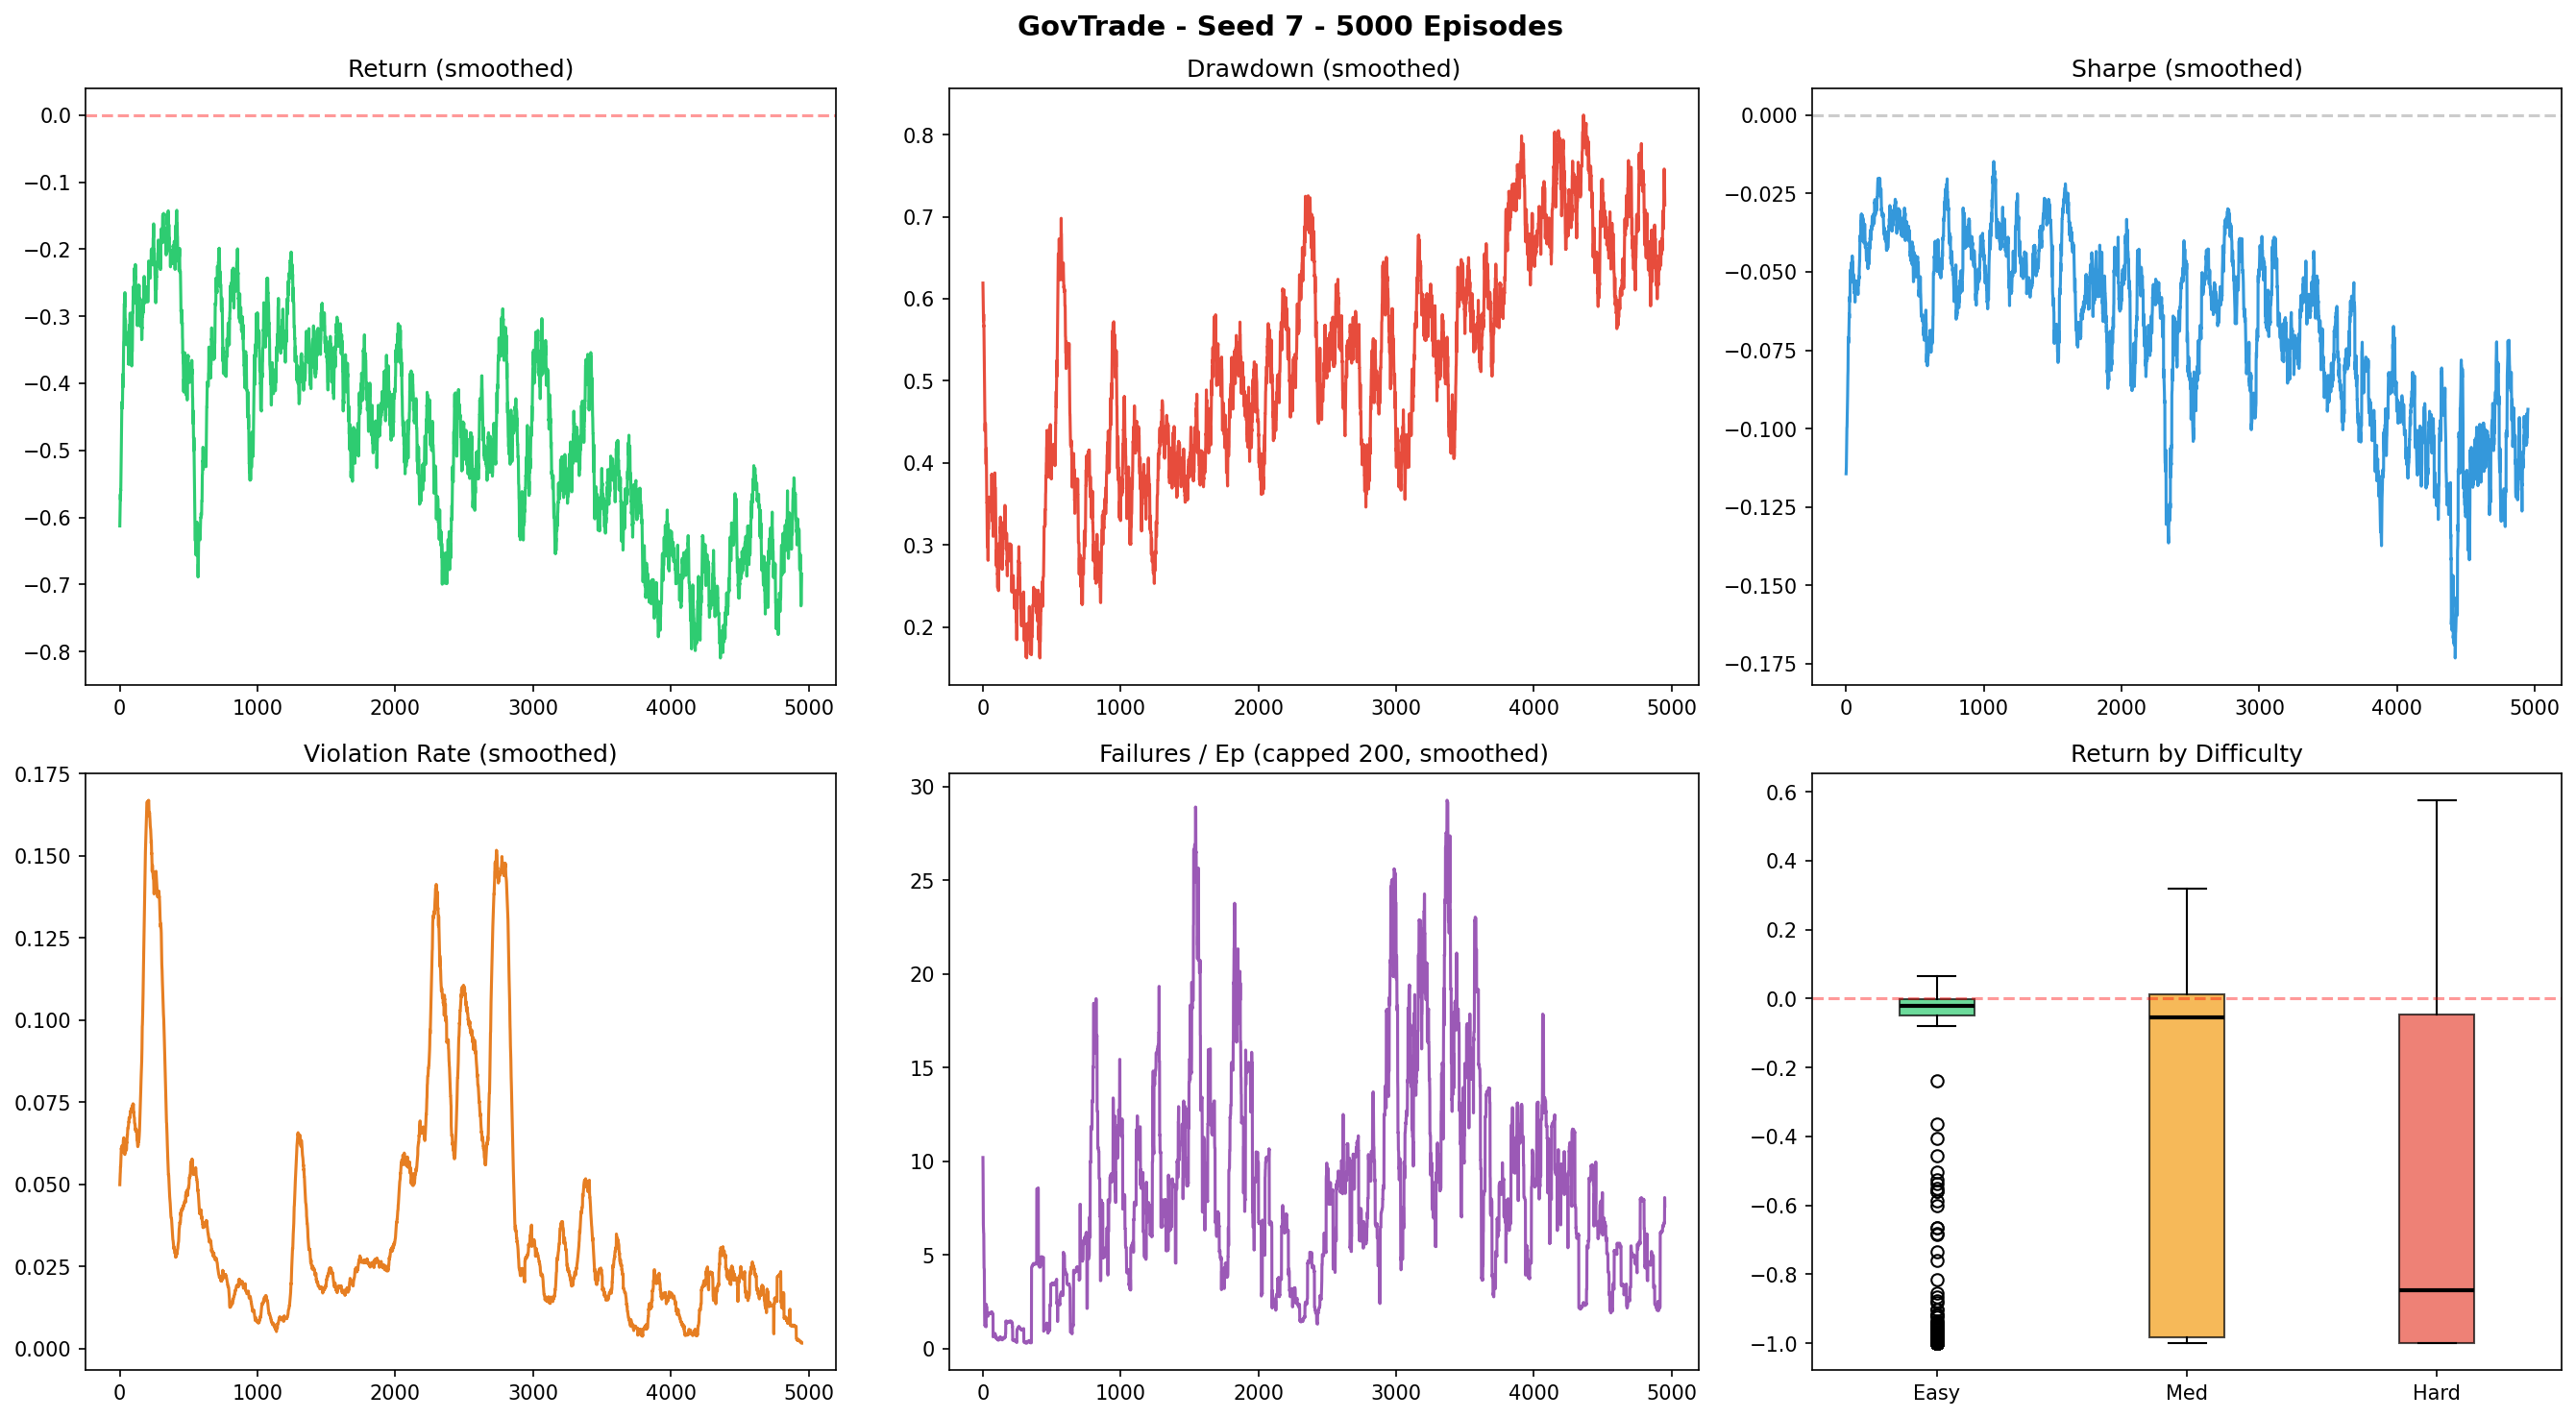
\includegraphics[width=1.0\textwidth]{figures/training_curves.png}
    \caption{Training curves for Seed 7 across 5{,}000 episodes. The alternating optimization cycle (Trader $\rightarrow$ RM $\rightarrow$ PM, 50 episodes each) produces characteristic oscillation patterns as each agent adapts to its counterparts' frozen policies. The best Governance Score of 0.8009 was achieved at episode 4{,}727.}
    \label{fig:training_curves}
\end{figure}

\begin{figure}[h]
    \centering
    \includegraphics[width=\textwidth]{figures/governance_score_distribution.png}
    \caption{Distribution of Best Governance Scores across all nine training seeds. The violin plot shows the full spread; individual seeds are overlaid as colored points. The 95\% confidence interval of the mean is shaded in orange. The distribution is approximately unimodal with mild left skew, driven by the two Low-category seeds (4 and 42).}
    \label{fig:score_dist}
\end{figure}

% ═══════════════════════════════════════════════════════════════════════════
\clearpage
\bibliographystyle{unsrt}
\bibliography{references}

% ═══════════════════════════════════════════════════════════════════════════
\appendix
\section{Hyperparameters}
\label{app:hyperparams}

\begin{table}[h]
\centering
\begin{tabular}{@{}ll@{}}
\toprule
\textbf{Parameter} & \textbf{Value} \\ \midrule
PPO clip $\epsilon$ & 0.2 \\
GAE $\lambda$ & 0.95 \\
Discount $\gamma$ & 0.99 \\
Learning rate (all agents) & $3 \times 10^{-4}$ \\
PPO epochs per update & 4 \\
Minibatch size & 64 \\
Hidden layers & 3 $\times$ 256 \\
Activation & GELU \\
Layer normalization & Yes \\
Entropy coefficient (initial) & 0.01 \\
Entropy decay & 0.9998 \\
Max gradient norm & 0.5 \\
Phase length (alternating) & 50 episodes \\
Total episodes per seed & 5{,}000 \\
Max steps per episode & 500 \\
Initial cash & \$100{,}000 \\
Commission & 0.1\% \\
Ticket fee & \$5.00 \\
RM size limit floor & 0.20 (DD $< 15\%$) \\
PM capital floor & 0.15 (DD $< 20\%$) \\
\bottomrule
\end{tabular}
\caption{Complete hyperparameter specification.}
\label{tab:hyperparams}
\end{table}

\end{document}


